%%%%%%%%%%%%%%%%%%%%%%%%%%%%%%%%%%%%%%%%%%%%%%%%%%%%%%%%%%%%%%%%%%%%%%%%%%%%%%%%%%%%%%%%%%%%%%%%%%%%%%%%%%%%%%%%%%%%%%
\chapter{Compare time integration methods}
%%%%%%%%%%%%%%%%%%%%%%%%%%%%%%%%%%%%%%%%%%%%%%%%%%%%%%%%%%%%%%%%%%%%%%%%%%%%%%%%%%%%%%%%%%%%%%%%%%%%%%%%%%%%%%%%%%%%%%
%!!!!!!!!!!!!!!!!!!!!!!!!Endre $y$( $u$ eller $U$) til noe annet!!!!!!!!!!!!!!!!!!!!\\
This section will be concerned with comparing the integrators. How well they estimate the error and energy will be the primary concern.\\

The relevant integrators are trapezoidal rule, forward euler, and midpoint rule. The definition, and the iteration scheme, of the different methods are given in the table below. 

\begin{table}
\begin{tabular}{l l l}
	Trapezoidal rule \cite{trapezoidal} & $U_{i+1} = U_{i}+h_t g \Big( \frac{1}{2}(t_i+t_{i+1}),\frac{1}{2}(U_i+U_{i+1}) \Big)$ & 
	$U_{i+1} = (I- \frac{A h_t}{2})\backslash \Big(  U_i + \frac{h_t}{2} \big( A U_i+(F_{i+1}+F_i) \big)  \Big) $\\
	Forward Euler \cite{forwardeuler} & $ U_{i+1} = U_i + h_t g ( t_i, U_i ) $ & $ U_{i+1} = U_i + h_t \big( A U_i + F_i \big) $ \\
	Midpoint rule \cite{midpoint} & $U_{i+2} = y_i + h_t + g \Big(  t_{i+1} , \frac{1}{2}(U_i + U_{i+2})    \Big) $ & 
	$U_{i+2} = ( I - A h_t )\backslash \Big( U_i + 2h_t \big( \frac{A U_i}{2} + F_{i+1} \big) \Big) $ \\
\end{tabular}
\label{tab:intmet}
\caption{ Proposed methods for integrating in time. A problem that arises with the midpoint rule is the need to know $F_{i+\frac{1}{2}}$, this is solved by doubling the step size. Er denne tabellen fin nok?}
\end{table}

Convergence of the different methods are shown in figure \ref{fig:intconv}

\begin{figure}[H]
        \centering
        \begin{subfigure}[b]{0.30\textwidth}
                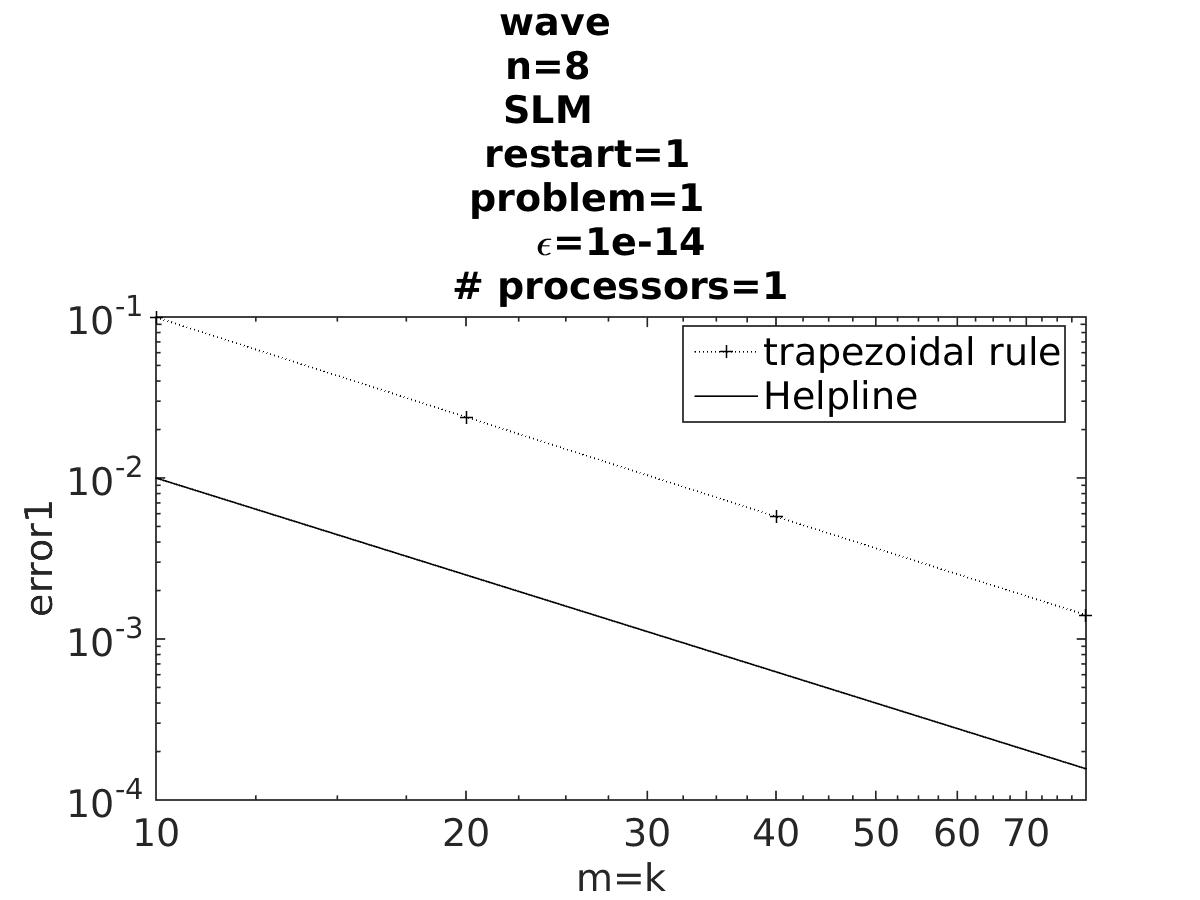
\includegraphics[width=\textwidth]{../MATLAB/fig/intconvtrap.jpg}
                %\includegraphics[width=\textwidth]{test}
                \caption{ Help line decreases with $m^2$. }
                \label{fig:intconvtrap}
        \end{subfigure}%
        ~
        \begin{subfigure}[b]{0.30\textwidth}
                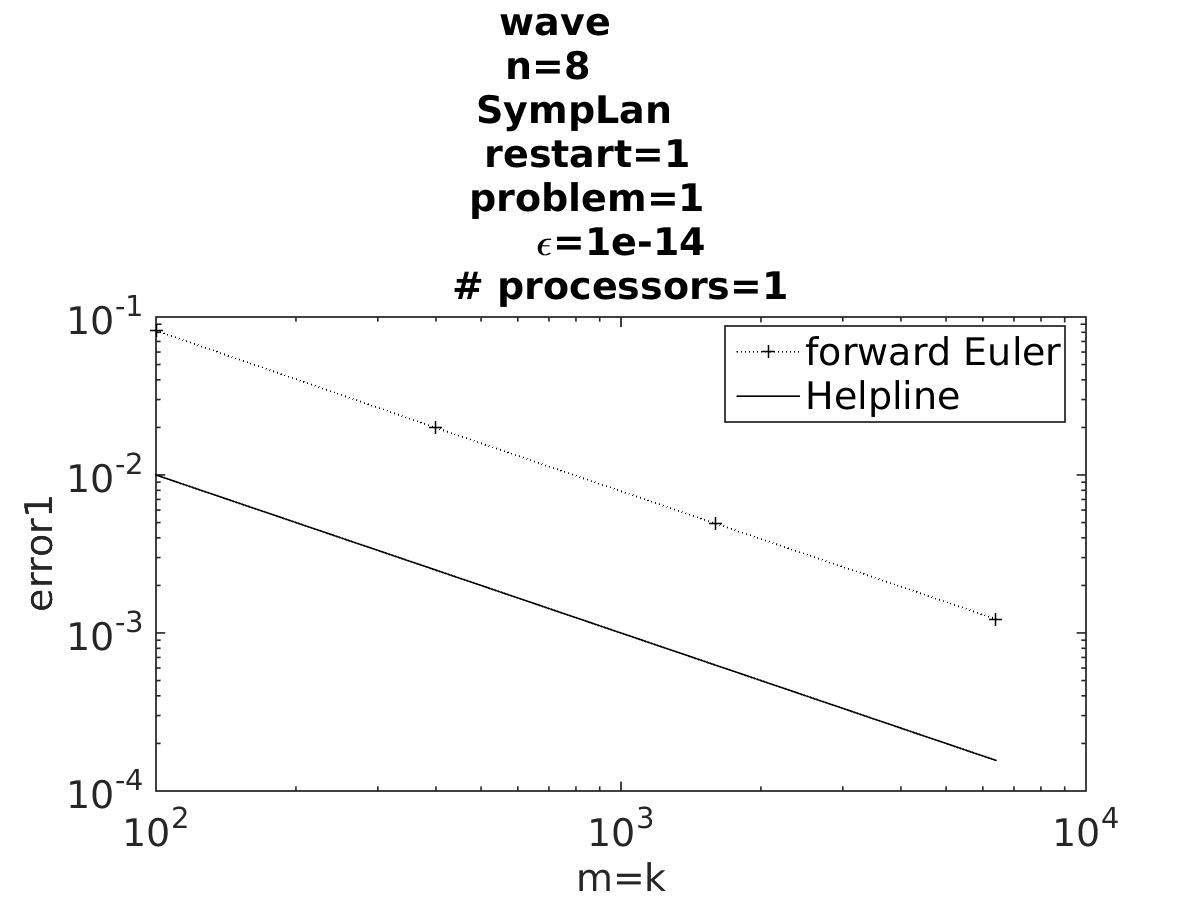
\includegraphics[width=\textwidth]{../MATLAB/fig/intconveul.jpg}
                %\includegraphics[width=\textwidth]{test}
                \caption{ Help line decreases with $m$. }
                \label{fig:intconveul}
        \end{subfigure}
        \begin{subfigure}[b]{0.30\textwidth}
                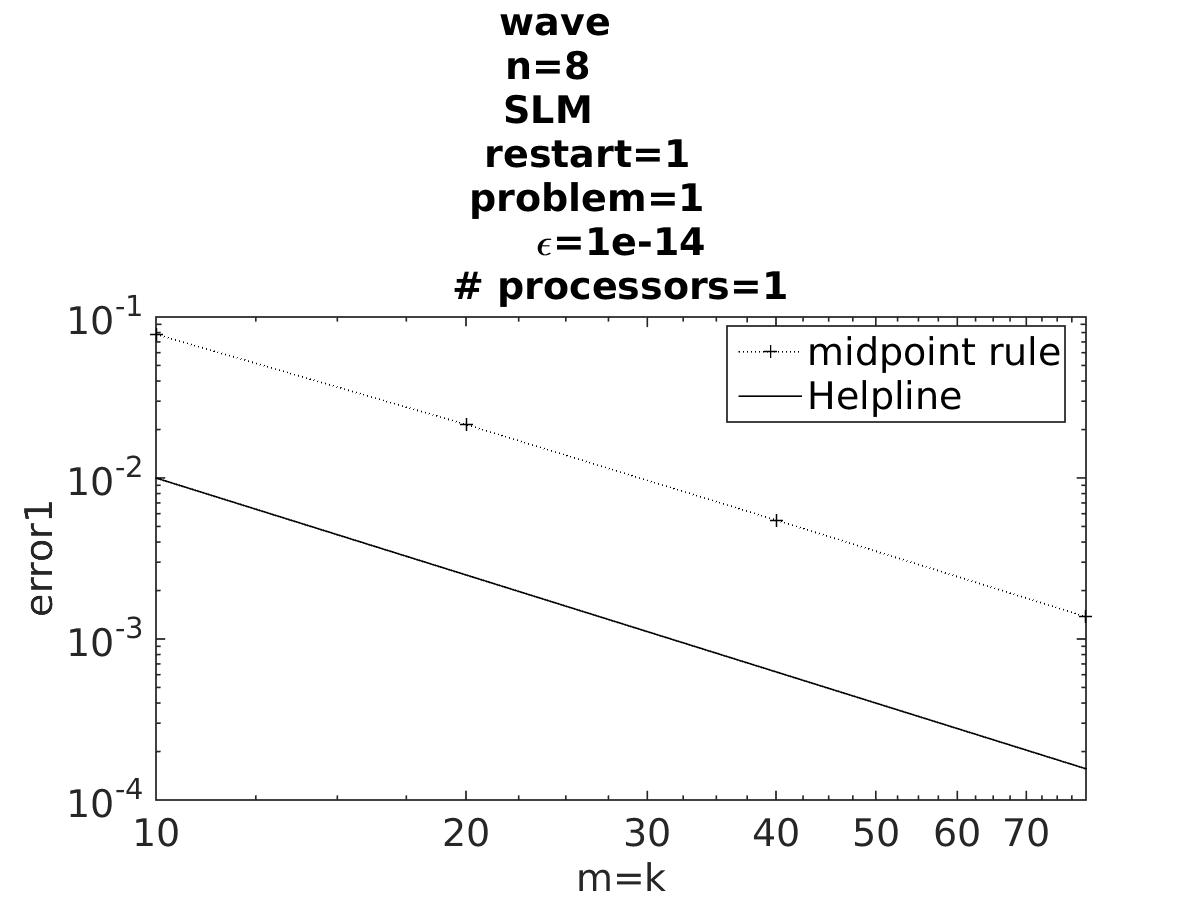
\includegraphics[width=\textwidth]{../MATLAB/fig/intconvmid.jpg}
                %\includegraphics[width=\textwidth]{test}
                \caption{ Help line decreases with $m^2$. }
                \label{fig:intconvmid}
        \end{subfigure}
        \caption{Figure of the convergence for the different integration methods. All methods converge with the expected rate. }
        \label{fig:intconv}
\end{figure}


\begin{figure}[H]
        \centering
        \begin{subfigure}[b]{0.30\textwidth}
                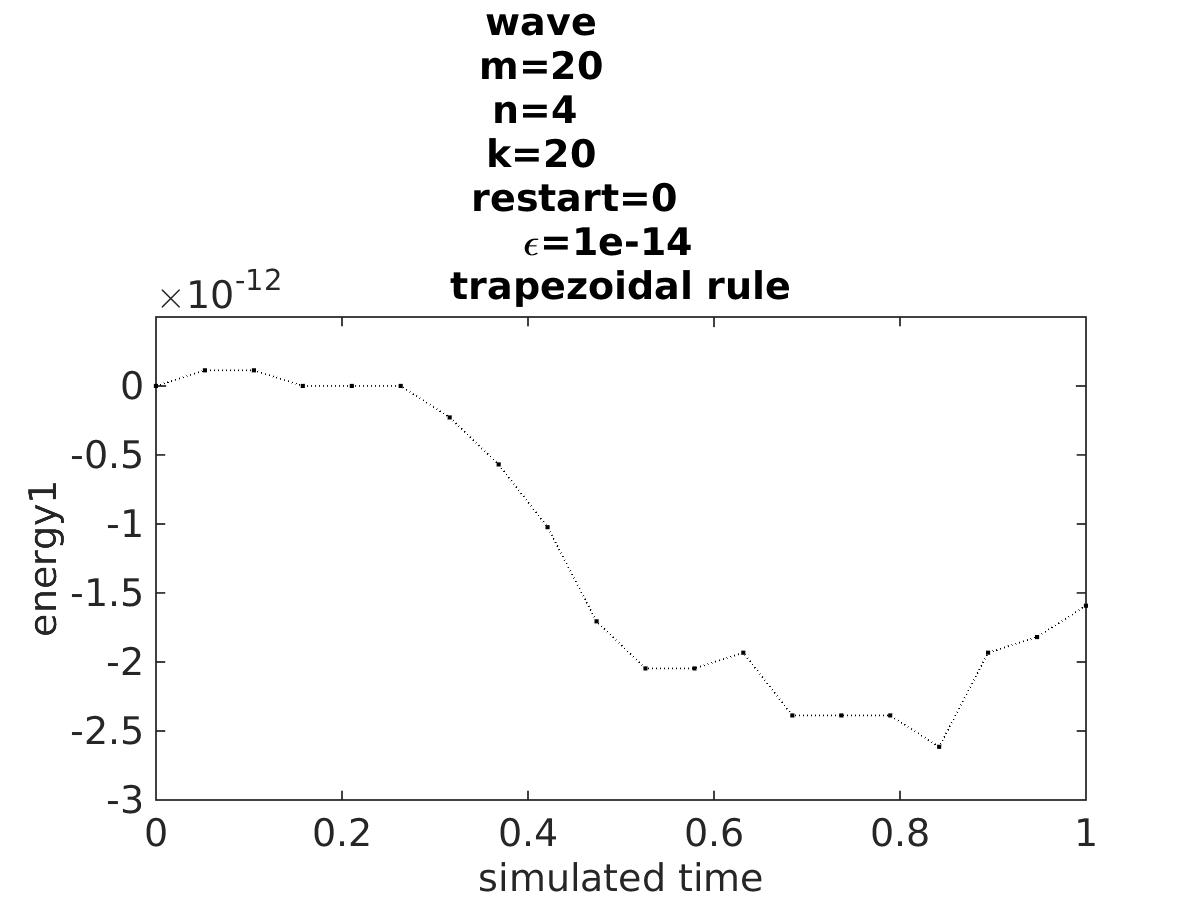
\includegraphics[width=\textwidth]{../MATLAB/fig/energyovertimetrapezoidal.jpg}
                \caption{  }
                \label{fig:errortrap}
        \end{subfigure}%
        ~
        \begin{subfigure}[b]{0.30\textwidth}
                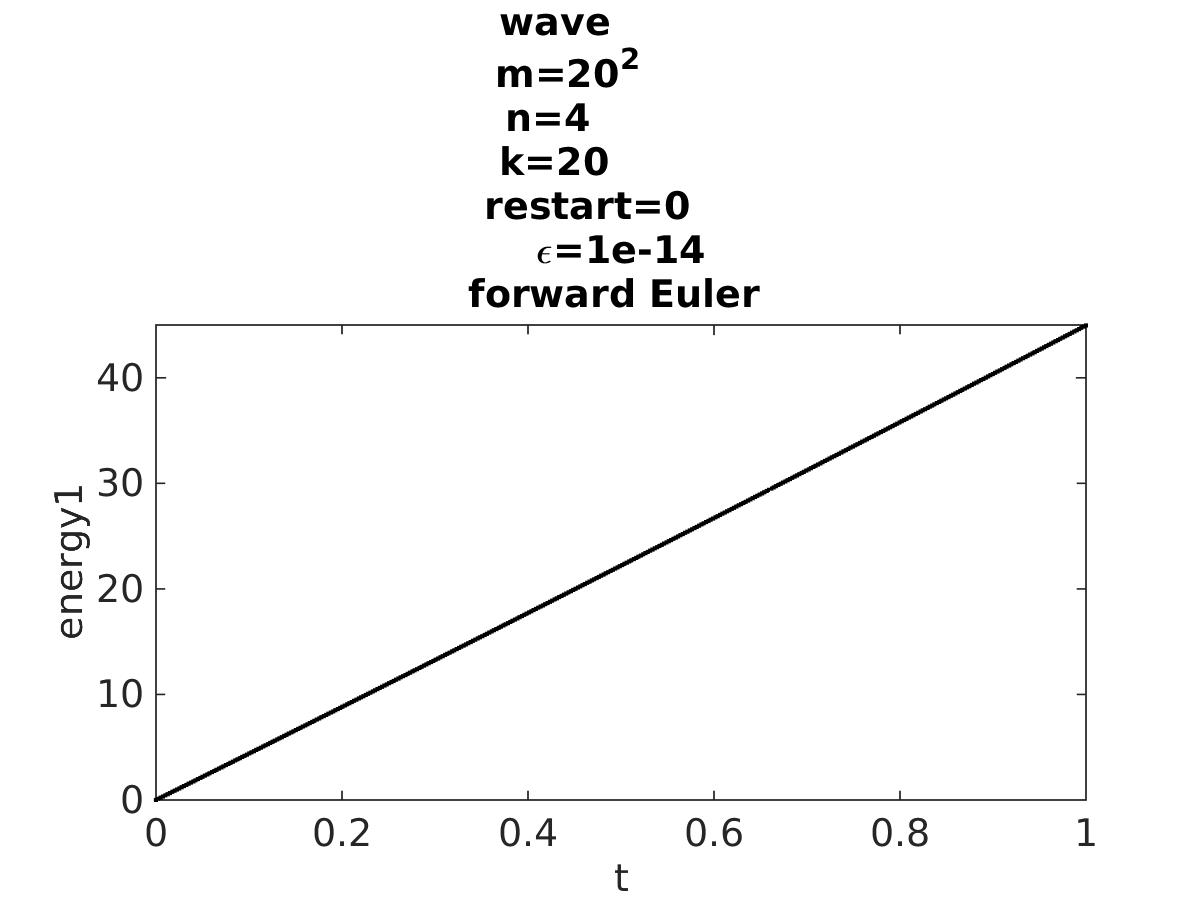
\includegraphics[width=\textwidth]{../MATLAB/fig/energyovertimeeuler.jpg}
                \caption{  }
                \label{fig:erroreul}
        \end{subfigure}
        \begin{subfigure}[b]{0.30\textwidth}
                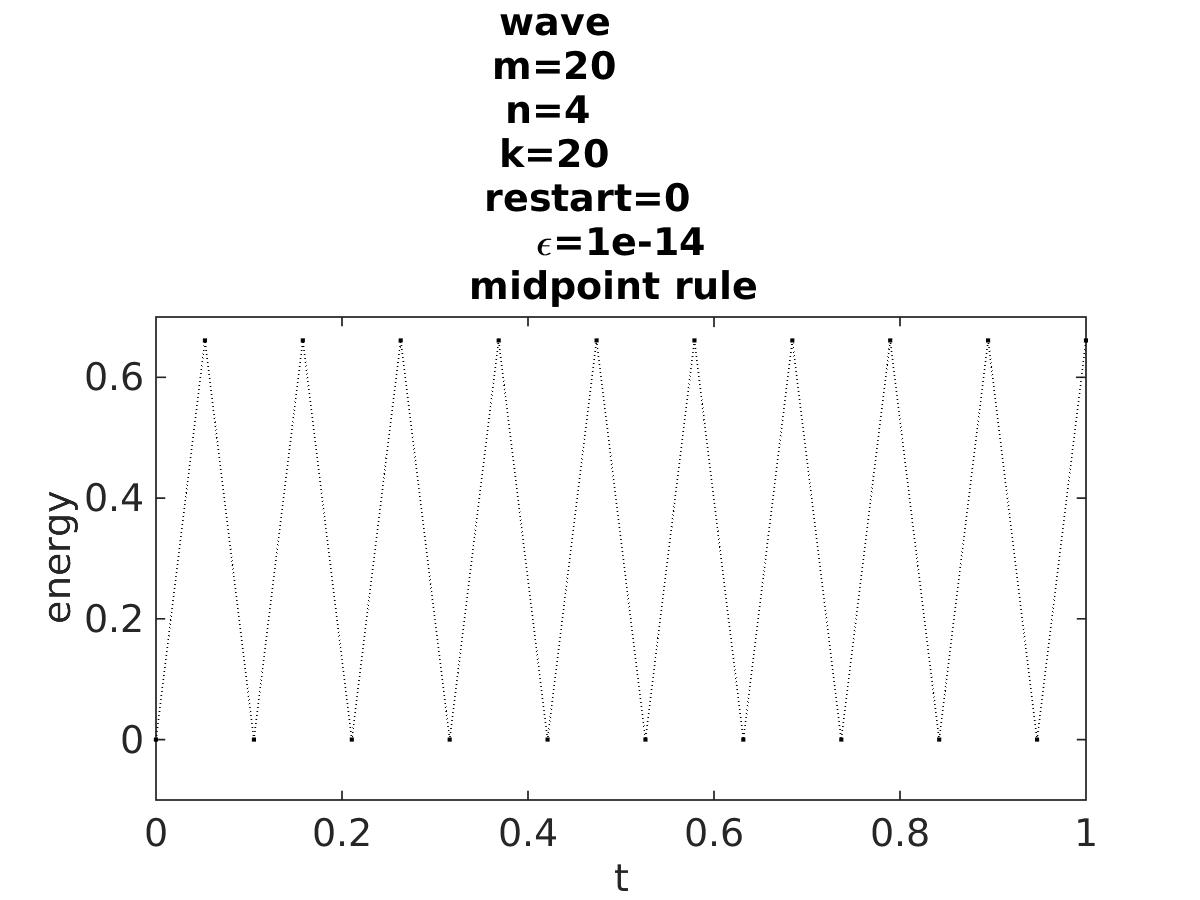
\includegraphics[width=\textwidth]{../MATLAB/fig/energyovertimemidpoint.jpg}
                \caption{  }
                \label{fig:errormid}
        \end{subfigure}
        \caption{Figure of the difference in energy at a point in time. It is clear that only trapezoidal rule gives a suitable approximation of the error. Forward euler has an linearly increasing energy, while the midpoint rule gives periodic energy.}
        \label{fig:error}
\end{figure}
After looking at figure \ref{fig:error} it is easy to conclude that trapezoidal rule outperforms the other two integration methods.